\chapter{C 編譯器}
  c 語言是當年寫unix系統kernel的母語,system call API的形式也是c語言,所以
  當初opensource最重要的關鍵創作就是這個底層基本工具。有了c 編譯器,則所有
  用c API寫的程式,只要想辦法重新在新系統編譯過,那就有相同的應用程式可以
  用了。GNU當年為了能快速利用一個系統,所以痛定思痛下,決定做出一個 C
  compiler,是為gcc。現在則是所有相關的編譯程式例如fortran編譯器,
  都為gcc下的一個子單位。
  \\\\
  c經過這麼多年的發展,有很多實作與變化,就像語言一樣,即使是閩南語,也有分
  泉州,漳州,廈門等口音不同,c也有很多細微不同的標準,例如ANSI C,C99標準
  等,gcc也有加入一些他們特有的features,這也都是更深入時要稍微小心的。
  \section{基本使用}
  一個編譯過程通常需要4道程序
  \begin{itemize}
    \item preprocess	先處理那些\verb=#ifdef #define=這些東西並做一些巨集代換
    \item compile	做語意分析,翻譯成組合語言
    \item assemble	翻成機器碼與OS有關的格式,做成relocatable obj檔。
    \item link  	找到symbol(函式,變數名)與程式庫(libary)中的副程式
                        ,做成可執行obj檔(executable obj)。
  \end{itemize}
  分別由cpp,cc1,as,ld來完成。但我們通常用個
  \begin{verbatim}
  $ gcc xxx.c
  \end{verbatim}
  就好了,這是因為
  gcc或者g++只是個編譯驅動器(compiler driver),這個驅動器去叫cpp這些工具來完成
  編譯過程中所需要的步驟。其中as, ld這些工具又放在另一個package叫binutils的裡面
  ,所以要裝好gcc,不僅要gcc的套件,連binutils 這個套件都要小心。另外更重要的
  是函式庫的版本與kernel的版本(安裝gcc要小心很多東西,像gpref也要更新成有support)
  。\\\\
  重要的選項或旗標(FLAGS),一些基本用到的編譯選項,如下
  \begin{verbatim}
-c: 只建立obj檔,留待後面才來連結(link)
-S: 只建立assemblely檔。
-g: 建立一些除錯資訊給可執行檔,這樣debug工具ddd,gdb才能除錯。
-o: 把建立的二位元檔給另外名字,因為可執行檔最後內定名字是a.out。
-D: 條件編譯,搭配#ifdef #define用。如果有defined才編譯
-W: 編譯時出錯時,顯示錯誤訊息的條件。
-L: 給連結時要用到的靜態函式庫(static library)的搜尋目錄。
-I: 標頭檔.h的搜尋目錄。
-l: 正常連結只會在libc這個函數庫,其他靜態函數庫需要用這個指定連結。
-Wa: 傳給assembler as的參數
-Wp: 傳給preprocess cpp的參數
-Wl: 傳給linker ld的參數
-O1 -O2 -O3: 最佳化,會根據CPU的架構編出好的程式碼,需要多一點編譯時間。
	     -O2  是不錯的選擇。

      像這樣的例子
      
$ gcc -c -o test.o test.c
$ gcc -S -o test.s test.c
$ gcc -g -o test.o test.c
$ gcc -D_SOLARIS_ -o test test.c
$ gcc -Wall -L./lib/ -I./include/ -o foo.o foo.c
$ gcc -Wall -L../lib -I../include -lX11 -lXext -lm -o xprog xprog.c

  W用all表示所有的編譯warning都要秀出來。
  \end{verbatim}

  \section{標頭檔與函式庫}
  當我們給
  \begin{verbatim}
  $ gcc -c -o foo.o foo.c
  \end{verbatim}
  gcc怎麼知道去哪裡找foo.c裡面所include的header檔,連結函式庫
  與系統定義呢? 總共有下列來源指定gcc去那找。
  \begin{itemize}
    \item 用-D -I -L指定的(編譯時候)
    \item 當初在編譯gcc時指定的。
    \item 寫在gcc specs內的
    \item gcc根據環境變數設定(編譯的時候)
  \end{itemize}
  在shell下用這行,-E 表示只做到preprocess就好
  {\scriptsize
  \begin{verbatim}
  $ echo 'main(){}' | gcc -E -v -
Using built-in specs.
COLLECT_GCC=gcc Target: x86_64-linux-gnu
  \end{verbatim}
  \parbox{\textwidth}
{Configured with: ../src/configure -v --with-pkgversion='Debian 4.9.1-14' --with-bugurl=file:///usr/share/doc/gcc-4.9/README.Bugs --enable-languages=c,c++,java,go,d,fortran,objc,obj-c++ --prefix=/usr --program-suffix=-4.9 --enable-shared --enable-linker-build-id --libexecdir=/usr/lib --without-included-gettext --enable-threads=posix --with-gxx-include-dir=/usr/include/c++/4.9 --libdir=/usr/lib --enable-nls --with-sysroot=/ --enable-clocale=gnu --enable-libstdcxx-debug --enable-libstdcxx-time=yes --enable-gnu-unique-object --disable-vtable-verify --enable-plugin --with-system-zlib --disable-browser-plugin --enable-java-awt=gtk --enable-gtk-cairo --with-java-home=/usr/lib/jvm/java-1.5.0-gcj-4.9-amd64/jre --enable-java-home --with-jvm-root-dir=/usr/lib/jvm/java-1.5.0-gcj-4.9-amd64 --with-jvm-jar-dir=/usr/lib/jvm-exports/java-1.5.0-gcj-4.9-amd64 --with-arch-directory=amd64 --with-ecj-jar=/usr/share/java/eclipse-ecj.jar --enable-objc-gc --enable-multiarch --with-arch-32=i586 --with-abi=m64 --with-multilib-list=m32,m64,mx32 --enable-multilib --with-tune=generic --enable-checking=release --build=x86\_64-linux-gnu --host=x86\_64-linux-gnu --target=x86\_64-linux-gnu}
  \begin{verbatim}
Thread model: posix
gcc version 4.9.1 (Debian 4.9.1-14) 
COLLECT_GCC_OPTIONS='-E' '-v' '-mtune=generic' '-march=x86-64'
  \end{verbatim}
\parbox{\textwidth}{/usr/lib/gcc/x86\_64-linux-gnu/4.9/cc1 -E -quiet -v -imultiarch x86\_64-linux-gnu - -mtune=generic -march=x86-64}
\parbox{\textwidth}{ignoring nonexistent directory "/usr/local/include/x86\_64-linux-gnu"}
\parbox{\textwidth}{ignoring nonexistent directory "/usr/lib/gcc/x86\_64-linux-gnu/4.9/../../../../x86\_64-linux-gnu/include"}
  \begin{verbatim}
#include "..." search starts here:
#include <...> search starts here:
 /usr/lib/gcc/x86_64-linux-gnu/4.9/include
 /usr/local/include
 /usr/lib/gcc/x86_64-linux-gnu/4.9/include-fixed
 /usr/include/x86_64-linux-gnu
 /usr/include
End of search list.
# 1 "<stdin>"
# 1 "<built-in>"
# 1 "<command-line>"
# 1 "/usr/include/stdc-predef.h" 1 3 4
# 1 "<command-line>" 2
# 1 "<stdin>"
main(){}
  \end{verbatim}
\parbox{\textwidth}{COMPILER\_PATH=/usr/lib/gcc/x86\_64-linux-gnu/4.9/:/usr/lib/gcc/x86\_64-linux-gnu/4.9/:/usr/lib/gcc/x86\_64-linux-gnu/:/usr/lib/gcc/x86\_64-linux-gnu/4.9/:/usr/lib/gcc/x86\_64-linux-gnu/}
\parbox{\textwidth}{LIBRARY\_PATH=/usr/lib/gcc/x86\_64-linux-gnu/4.9/:/usr/lib/gcc/x86\_64-linux-gnu/4.9/../../../x86\_64-linux-gnu/:/usr/lib/gcc/x86\_64-linux-gnu/4.9/../../../../lib/:/lib/x86\_64-linux-gnu/:/lib/../lib/:/usr/lib/x86\_64-linux-gnu/:/usr/lib/../lib/:/usr/lib/gcc/x86\_64-linux-gnu/4.9/../../../:/lib/:/usr/lib/}
  \begin{verbatim}
COLLECT_GCC_OPTIONS='-E' '-v' '-mtune=generic' '-march=x86-64'
  \end{verbatim}}
  你會看到gcc當初編譯時用的選項,enable-shared --libdir=/usr/lib等等,
  而且header搜尋順序是/usr/local/include比/usr/include要先。並且會
  去讀 specs 檔,在我的debian系統上,在\verb=/usr/lib/gcc/x86_64-linux-gnu/4.9=
  下面,有很重要的一些specs檔案,裏面記載了要link的library名稱。以前所有的
  spec寫在一個檔案內,現在用
  \begin{verbatim}
  gcc -dumpspecs
  \end{verbatim}
  才會知道所有的內部規定是怎樣。
  \\\\
  函式庫在定義上是包含一堆編譯出來的object檔的集合archives檔,通常就是libxxx.a
  ,這libxxx.a裏面藏了很多xxx.o檔,這是靜態函式庫。而函式庫的搜尋與連結例如
  當我們用到數學函式cos(),cos這個symbol,gcc並不曉它到底是什麼東西,
  是變數,是函式,要預留多少空間給他等等,完全沒有任何訊息,你必須標頭
  檔要\verb=#include <math.h>=,gcc才知道。而且因為specs這個檔裡面只有要
  link -lc也就是只有libc.so這個檔內的symbol會被蒐尋,
  像printf scanf等都在這裡面,可是像cos()等就沒有了,
  所以函式庫的選項要多加 -lm ,這時ld才會來找libm這個函式庫,
  編譯的時候,gcc會去找-L,再找gcc的環境變數LIBRARY\_PATH,再找內定目錄
  /lib /usr/local/lib /usr/lib 這是當初compile gcc時寫在程式內的,
  gcc環境變數與pass給ld的機制在~gcc/gcc/collect2.c下找得到。
  這上面只是搜尋路徑而已,如果要不加-lm也能正確的主動搜尋某個特定的lib,
  例如libm,就要去在specs這個檔案改一下,把math這個函式庫加進自動聯結函式庫
  之一,就不用寫-lm了。
  \\\\
  因此在做連結時,object 檔的順序也是很重要的,如果在 link 時,看到
  undefined reference to 的錯誤,那可能是  link 的 .o 檔順序出了問題,而不是
  真的找不到 symbol。

  \section{靜態與動態連結執行檔}
    當我們產生執行檔時,ld會根據找到的.o .a檔裏面的function, symbol,把有用到的
    東拿一個西拿一點產生可執行的執行檔,這執行檔是根據OS, 機器cpu指令,統一檔案
    格式等規定所寫成的。這就是一般的靜態 (static) 執行檔。但這樣會浪費硬碟上的
    儲存空間,因為例如一個程式用到printf,另一程式也用到printf,但printf的程式
    碼其實一直都在/lib/x86\_64-linux-gnu/libc.a裏面啊,那每一隻程式都抄一份到
    自己的執行檔去就浪費了,所以後來就有動態連結,也就是link這個動作到執行
    (loading) 時才去做,執行檔裏面並沒有真正的code,只有一個參照訊息說這printf
    要找到一個 libc.so的檔才行執行。
    \\\\
    現在Linux系統內定都是使用動態編譯,所以如果編譯時沒有指定-static這個選項,
    其實可執行檔並不是真的可執行檔,它必須在執行(run time) 時需要 ld.so 或
    ld-linux.so來做最後的連結動作,建造一個可執行的 image丟到記憶體。
    \\\\
    當然真正的static/dynamic link沒有這麼簡單,也會根據linker的實作有所不同,
    也就是static link時,他並沒有把整個library copy進來,但也不是只有copy所呼叫
    到的程式碼,GNU linker的作法是copy的單位為object module,也就是如果func1, 
    func2, func3在func.o裏面,即使只有呼叫func1,那所有的func1, func2, func3都
    會copy到執行檔來,如果func1在func1.o, func2在func2.o, func3在func3.o,則
    只會copy func1到執行檔來。這會跟解開library的連結時間,與模組集中管理原則
    有關,所以這有trade-off,也可能是不同編譯器有不同想法與實作。
    \\\\
    這libc.so 是shared object也有人稱為dynamic lib, 跟libc.a不同的是libc.a裏面
    的機器碼一個很大的問題是mov, jump等指令組譯出來時,是含有記憶體位址的,這
    些記憶體位址被link到新的執行檔時,是要做 relocate 的計算的,也就是原本組語
    操作的記憶體位址,到新執行檔後是會變掉的。一個函式在一個.o檔要呼叫另一函式
    在另一.o檔,static lib使用symbol來參照,linker碰到這個symbol,就計算後
    換上一個記憶體位址,寫進執行檔去。
    \\\\
    而shared obj則是裏面的機器碼是通通放在一個固定的記憶體位址上,執行時loader
    叫dynamic linker ld.so ld-linux.so來尋找dynamic lib。找到後根據檔案系統與
    系統page fault的設定,把某段檔案內容載入到記憶體中,所以他的記憶體位址是
    最後才知道的,雖然也要重新計算但跟 static 是不一樣的。
    \\\\
    以下用3個API, myprint, myecho跟myprinter玩玩
    \begin{verbatim}
    test.c
#include <stdio.h>

int myprint()
{
        printf("haha\n");
}
int myecho()
{
        printf("hehe\n");
}

    test1.c
#include <stdio.h>

int myprinter()
{
        printf("hoho\n");
}

    myprint.c
#include <stdio.h>

int main()
{
        myprint();
        myprinter();
}
    \end{verbatim}
    然後用-c -o來產生static object檔
    \begin{verbatim}	
gcc -c -o test.o test.c
gcc -c -o test1.o test1.c
    \end{verbatim}
    用ar做archive檔
    \begin{verbatim}	
ar rc libtest.a test.o test1.o
    \end{verbatim}
    用-fPIC來編譯position independent code,準備做shared library
    \begin{verbatim}
gcc -fPIC -c -o test.o test.c
gcc -fPIC -c -o test1.o test1.c
    \end{verbatim}
    用-shared產生shared object
    \begin{verbatim}
gcc -shared -o libtest.so test.o test1.o
    \end{verbatim}
    如果-L目錄內同時有static跟dynamic的,目前內定是以dynamic為主,所以我們
    把libtest.a copy到static這個目錄,libtest.so copy到dynamic這個目錄下。
    當c程式有main()這個函式時,就要跟libtest來連結。分別產生兩個執行檔。
    \begin{verbatim}
gcc myprint.c -o sprint -Lstatic -ltest
gcc myprint.c -o dprint -Ldynamic -ltest
    \end{verbatim}
    如果同時兩個lib都在同一目錄下,就要用-Wl指定static
    \begin{verbatim}
gcc myprint.c -Wl,-static -o sprint -ltest
    \end{verbatim}
    其中-fPIC選項是很重要的選項,PIC表示position independent code,
    shared obj函式庫裡的程式碼為(PIC),也就是它的位址可能會隨著不同 process
    而有不同,例如我一個程式只用了libc.so ld-linux.so,通常這時後libc.so是從
    0x40017000開始的,但如果我一個程式用了libc.so ld-linux.so libm.so,則
    libc.so從 0x40034000 開始,兩個的printf參照,就會有不同的位址,所以像這
    種動態函式庫的內部資料就要說明這些code是PIC。
    \\\\
    他有兩種記憶體模式,small/large模式,small program symbol必須linked在2g以下
    我們使用-fPIC是large模式。
    \\\\
    使用ldd來看他們的差異
    \begin{verbatim}
chuang@dsuen-lnx:~$ ldd sprint 
        linux-vdso.so.1 (0x00007fff0a3fc000)
        libc.so.6 => /lib/x86_64-linux-gnu/libc.so.6 (0x00007f5745623000)
        /lib64/ld-linux-x86-64.so.2 (0x00007f57459e6000)
chuang@dsuen-lnx:~$ ldd dprint
        linux-vdso.so.1 (0x00007f0f16ece000)
        libtest.so => not found
        libc.so.6 => /lib/x86_64-linux-gnu/libc.so.6 (0x00007f0f16b0b000)
        /lib64/ld-linux-x86-64.so.2 (0x00007f0f16ed2000)
    \end{verbatim}
    動態的找不到libtest.so,所以export LD\_LIBRARY\_PATH=\$PWD/dynamic,可以
    看到 libtest.so會被放到0x00007fff071e0000,而相關的myprint, myecho, 
    myprinter都相對於這個位址。反之用libtest.a編譯的,myprint, myecho會被放到
    sprint裏面去,位址也跟動態的不同。
    \begin{verbatim}
chuang@dsuen-lnx:~$ export LD_LIBRARY_PATH=dynamic/
chuang@dsuen-lnx:~$ ldd dprint
        linux-vdso.so.1 (0x00007fff071e0000)
        libtest.so => dynamic/libtest.so (0x00007f4d9034f000)
        libc.so.6 => /lib/x86_64-linux-gnu/libc.so.6 (0x00007f4d8ff8e000)
        /lib64/ld-linux-x86-64.so.2 (0x00007f4d90552000)
    \end{verbatim}
    有趣的話,可以用nm對所有的.o .a .so dprint, sprint掃一遍位址,可以看出很多
    差異。
    \begin{verbatim}
chuang@dsuen-lnx:~$ nm sprint
0000000000600980 B __bss_start
0000000000600980 b completed.6661
0000000000600970 D __data_start
0000000000600970 W data_start
0000000000400440 t deregister_tm_clones
00000000004004c0 t __do_global_dtors_aux
0000000000600758 t __do_global_dtors_aux_fini_array_entry
0000000000600978 D __dso_handle
0000000000600768 d _DYNAMIC
0000000000600980 D _edata
0000000000600988 B _end
00000000004005b4 T _fini
00000000004004e0 t frame_dummy
0000000000600750 t __frame_dummy_init_array_entry
0000000000400748 r __FRAME_END__
0000000000600940 d _GLOBAL_OFFSET_TABLE_
                 w __gmon_start__
00000000004003a8 T _init
0000000000600758 t __init_array_end
0000000000600750 t __init_array_start
00000000004005c0 R _IO_stdin_used
                 w _ITM_deregisterTMCloneTable
                 w _ITM_registerTMCloneTable
0000000000600760 d __JCR_END__
0000000000600760 d __JCR_LIST__
                 w _Jv_RegisterClasses
00000000004005b0 T __libc_csu_fini
0000000000400540 T __libc_csu_init
                 U __libc_start_main@@GLIBC_2.2.5
0000000000400506 T main
0000000000400526 T myecho
0000000000400516 T myprint
                 U puts@@GLIBC_2.2.5
0000000000400480 t register_tm_clones
0000000000400410 T _start
0000000000600980 D __TMC_END__

    \end{verbatim}
    系統愈搞愈大,搜尋這麼多路徑跟函式庫也變成執行的瓶頸,
    所以每次有新改版程式或新加動態函式庫如果不在原本的/etc/ld.so.conf搜尋路徑
    中,都要把路徑加進來,然後用
        \begin{verbatim}
ldconfig -v 
        \end{verbatim}
    會重建cache並且顯示它所參照的函式庫。Run Time時ld.so才快速找得到lib"執行"。
    \\\\
    一些重要的程式
  \begin{itemize}
    \item ld 編譯用的linker, Link Editor 連結各obj寫進一個可執行檔(executable)。
    \item ldd 看obj檔由哪些shared obj組成
    \item ld.so 執行時的dynamic linker 負責 a.out格式。
    \item ld-linux.so 執行時的dynamic linker,負責elf格式。新的glicb2的
      ld-linux.so.2 已經跟ld.so.2結合成單一程式了
    \item ldconfig ld.so搜尋的cache, 根據/etc/ld.so.conf內的目錄,做出動態連結所
      需的 cache 檔。
  \end{itemize}
  一些重要的path設定與Makefile裏面常見的環境變數。
  \begin{itemize}
    \item -I include header search path
    \item -L library search path
    \item -lxxx link library name with libxxx.a or libxxx.so
    \item -M -MM -MD 這會把include中所需的.h 與c檔案dependency全列出來, -MD會
      導到一個.d檔去。這在make中常用來作為target的dependency列表,以利下次自動
      編譯。 -MM 會忽略 /usr/include的相依,只有你的程式header 相依檔會列出。
    \item -Wl,-rpath,/path/to/so 增加dynamic lib搜尋的目錄並特別寫進shared obj。
    \item -sysroot 指定/usr/lib /usr/include的相對根目錄。
          這可以使得多編譯環境在一個系統下同時存在。
  \end{itemize}
  -Wl,-rpath這個比較奇特一點,他有兩種選擇。-rpath與-rpath-link
  當link的so有其他dependancy so不在系統內定目錄時,-rpath-link不會寫進so
  -rpath會把絕對路徑寫進so檔。
  \begin{verbatim}
$ objdump -x libxxx.so | grep -i rpath
  \end{verbatim}
  這主要是在用./configure時,libtool搜尋時特定使用。
  根據man page的文件,重要的環境變數與gcc的使用有關的有
  \begin{itemize}
    \item C\_INCDLUE\_PATH c include header 搜尋路徑
    \item CPLUS\_INCLUDE\_PATH c++的include header搜尋路徑
    \item OBTC\_INCLUDE\_PATH objective C的include header搜尋路徑
    \item CPATH 
    \item LIBRARY\_PATH
    \item LD\_LIBRARY\_PATH 執行時,dynamic linker會去搜尋.so檔的path
  \end{itemize}
  有的是之後GNU Makefile或者是autoconf會特別用到的內定變數
  \begin{itemize}
    \item CC 使用的c編譯器,主要是當時各公司的電腦都有cc與gcc兩套編譯器。
    \item CPP 使用的前置header處理器,cpp是gcc用來處理.h檔的。
    \item LIBS 
    \item CFLAGS CXXFLAGS c, c++編譯時用的參數,通常是-I -D之類的。
    \item LDFLAGS 連結時用的參數,通常是-L, -l, -Wl之類的。
  \end{itemize}
    \subsection{dlopen與多樣性API選擇}
    在上面動態連結的library所產生的執行檔,用ldd看時,會顯示所有需要的動態程
    式庫,如果在搜尋目錄沒有的話,就無法執行,聽起來很合理,可是完成一件事,
    不見得是一定要使用某特別函式庫,例如security的ssl library,你可以使用
    openssl,也可以使用gnutls,只是不同的實作而已,再來就是例如視訊的使用,
    同樣解碼mpeg,可以用vdapu,或intel的va-api,那如果綁死某一個程式庫,寫
    進去執行檔就很固定,另外同樣api,也有可能版本稍微不同就要重來,所以使用
    dlopen去搜尋與開啟一個動態程式庫,根據他有的symbol,找到可以用的API,會讓
    程式寫作有更大的run time彈性。就好像要去高雄,看高鐵沒位子了,還可以用台鐵
    不會說一定要坐高鐵。不過就是你要熟悉不同的API,就像要熟悉不同的買票系統。

  \section{binutils的使用}
  binutils是一定伴隨gcc,g++安裝時也會安裝的package。他主要是要處理object檔,
  所以有必要對object檔做一番了解。
    \subsection{elf檔案格式}
    object檔案是系統gcc編譯後的二進位檔的統稱,由於他也有統一的格式,
    就跟圖檔有jpg, gif檔的格式一樣。以前unix下的格式為coff檔,目前使用
    的格式為ELF格式,他有六種obj檔分類,比較常接觸到為以下的分類。
    \begin{itemize}
      \item relocatable :  這就是我們編譯時產生的.o檔
      \item executable  :  這就是我們最後的可執行檔
      \item shared obj  :  這就是在/lib /usr/lib下的那些可以動態連結的函式庫檔
      \item core        :  Core Dump時產生的檔案
    \end{itemize}
    除了code以外,這種檔有很多訊息是放在檔頭,以及sections裏面的,就像tcp/ip
    的header資訊一樣,他有很多額外的資訊提供給linker, loader來使用的。
    \begin{center}
    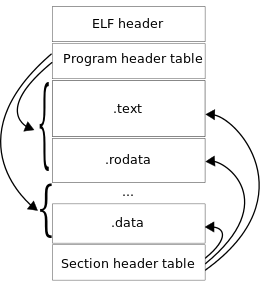
\includegraphics[width=8cm,height=10cm]{images/elf.png}
    \end{center}
    一個ELF OBJ檔隨著它存在的時期有不一樣的需求與組成名詞,在要連結linking時期
    躺在硬碟,包含了
    \begin{verbatim}
ELF header
program header table (可以不要)
section 0
section 1
section 2
section 3
section ...
section n
section header table
    \end{verbatim}
    ELF header 放了ELF所定義的一些例如ELF格式識別字串(俗稱magic number)
    ,還有是那種OBJ檔案type(shared obj, relocatable還是executable)等等
    這種general的資訊。
    \\\\
    program header table描述了一個segment的資訊,segment跟section不太一樣是屬
    於程式執行期的元素,所以在程式執行時期是必要的, 在連結時期是不必要的,
    所以如果你的程式不做連結動作只要有program table就好,
    \\\\
    section header table就是一個索引表來記錄各個section的索引
    \\\\
    sections就是把需要的資料根據屬性用途分門別類後的小集合,
    有.bss .data .init .debug .dynamic .fini .text ........,
    其中比較重要的
    \begin{description}%[align=right]
      \item [.fini] 裡面藏著finish的code,正常exit的code。
      \item [.init] 裡面藏著起始的code,也就是main開始的地方。
      \item [.text] 裡面就是真的CPU指令
      \item [*COM*] common section,只存在relocate object檔中,放沒有init的全域變數與extern 變數。
      \item [.bss] 在relocate object檔中,放有init的全域變數,在executable檔中,放沒有initialize的全域變數。
      \item [.data] 放有initialize的data
      \item [.debug] 放有可以讓gdb trace程式的資訊
      \item [.dynamic] 動態shared object的資訊
    \end{description}
    .bss, *COM*跟.data是一般比較混淆的地方,跟relocate, executable兩種檔案有關,
    要小心。 3 informations比較常用到
    \begin{itemize}
      \item symbol table 關於所有變數函式的參照table
      \item debug info 能讓gdb使用來trace的debug資訊。
      \item dynamic symbol table 給shared obj連結的資訊。
    \end{itemize}
    我們用小程式來看各 section 的儲存資料。
    \begin{verbatim}
#include <stdio.h>
#include <stdlib.h>

int global_a;
char global_b = 5;
static int global_c;
static char global_d = 5;
char *global_str0 = "string0";
char global_str1[] = "string1";
char global_array[3] = {1, 2, 3};

int func()
{
        int func_a;
}

int main()
{
        int main_a;
        char main_b = 15;
        static int main_c;
        static char main_d = 5;
        char *main_str0 = "str0";
        char main_str1[] = "str1";
        char main_array[3] = {1, 2, 3};
        int global_a;
        int *heap_a;

        heap_a = (int *) malloc(sizeof(int) * 4);
}
  \end{verbatim}
  用gcc -g mysection.c 編譯完後,使用objdump -x a.out 可以看出所有的header內容。
  可以看出來gcc對"執行檔"的設計是只有static 與 glboal 變數放在 .data .bss,有
  給值的放在.data,沒給值的放在.bss,全域func放在 .text 。.data裏面還可分可變
  read write 與不可變 read only 的變數。另外在relocate檔中的全域init與非init變數
  還有extern變數放的地方跟executable檔不太一樣。
  \begin{verbatim}

a.out:     file format elf64-x86-64
a.out
architecture: i386:x86-64, flags 0x00000112:
EXEC_P, HAS_SYMS, D_PAGED
start address 0x0000000000400410

Program Header:
    PHDR off    0x0000000000000040 vaddr 0x0000000000400040 paddr 0x0000000000400040 align 2**3
         filesz 0x00000000000001c0 memsz 0x00000000000001c0 flags r-x
  INTERP off    0x0000000000000200 vaddr 0x0000000000400200 paddr 0x0000000000400200 align 2**0
         filesz 0x000000000000001c memsz 0x000000000000001c flags r--
    LOAD off    0x0000000000000000 vaddr 0x0000000000400000 paddr 0x0000000000400000 align 2**21
         filesz 0x0000000000000734 memsz 0x0000000000000734 flags r-x
    LOAD off    0x0000000000000738 vaddr 0x0000000000600738 paddr 0x0000000000600738 align 2**21
         filesz 0x000000000000024c memsz 0x0000000000000260 flags rw-
 DYNAMIC off    0x0000000000000750 vaddr 0x0000000000600750 paddr 0x0000000000600750 align 2**3
         filesz 0x00000000000001d0 memsz 0x00000000000001d0 flags rw-
    NOTE off    0x000000000000021c vaddr 0x000000000040021c paddr 0x000000000040021c align 2**2
         filesz 0x0000000000000044 memsz 0x0000000000000044 flags r--
EH_FRAME off    0x00000000000005e4 vaddr 0x00000000004005e4 paddr 0x00000000004005e4 align 2**2
         filesz 0x000000000000003c memsz 0x000000000000003c flags r--
   STACK off    0x0000000000000000 vaddr 0x0000000000000000 paddr 0x0000000000000000 align 2**4
         filesz 0x0000000000000000 memsz 0x0000000000000000 flags rw-

Dynamic Section:
  NEEDED               libc.so.6
  INIT                 0x00000000004003a8
  FINI                 0x00000000004005c4
  INIT_ARRAY           0x0000000000600738
  INIT_ARRAYSZ         0x0000000000000008
  FINI_ARRAY           0x0000000000600740
  FINI_ARRAYSZ         0x0000000000000008
  GNU_HASH             0x0000000000400260
  STRTAB               0x00000000004002e0
  SYMTAB               0x0000000000400280
  STRSZ                0x000000000000003f
  SYMENT               0x0000000000000018
  DEBUG                0x0000000000000000
  PLTGOT               0x0000000000600928
  PLTRELSZ             0x0000000000000048
  PLTREL               0x0000000000000007
  JMPREL               0x0000000000400360
  RELA                 0x0000000000400348
  RELASZ               0x0000000000000018
  RELAENT              0x0000000000000018
  VERNEED              0x0000000000400328
  VERNEEDNUM           0x0000000000000001
  VERSYM               0x0000000000400320

Version References:
  required from libc.so.6:
    0x09691a75 0x00 02 GLIBC_2.2.5

Sections:
Idx Name          Size      VMA               LMA               File off  Algn
  0 .interp       0000001c  0000000000400200  0000000000400200  00000200  2**0
                  CONTENTS, ALLOC, LOAD, READONLY, DATA
  1 .note.ABI-tag 00000020  000000000040021c  000000000040021c  0000021c  2**2
                  CONTENTS, ALLOC, LOAD, READONLY, DATA
  2 .note.gnu.build-id 00000024  000000000040023c  000000000040023c  0000023c  2**2
                  CONTENTS, ALLOC, LOAD, READONLY, DATA
  3 .gnu.hash     0000001c  0000000000400260  0000000000400260  00000260  2**3
                  CONTENTS, ALLOC, LOAD, READONLY, DATA
  4 .dynsym       00000060  0000000000400280  0000000000400280  00000280  2**3
                  CONTENTS, ALLOC, LOAD, READONLY, DATA
  5 .dynstr       0000003f  00000000004002e0  00000000004002e0  000002e0  2**0
                  CONTENTS, ALLOC, LOAD, READONLY, DATA
  6 .gnu.version  00000008  0000000000400320  0000000000400320  00000320  2**1
                  CONTENTS, ALLOC, LOAD, READONLY, DATA
  7 .gnu.version_r 00000020  0000000000400328  0000000000400328  00000328  2**3
                  CONTENTS, ALLOC, LOAD, READONLY, DATA
  8 .rela.dyn     00000018  0000000000400348  0000000000400348  00000348  2**3
                  CONTENTS, ALLOC, LOAD, READONLY, DATA
  9 .rela.plt     00000048  0000000000400360  0000000000400360  00000360  2**3
                  CONTENTS, ALLOC, LOAD, READONLY, DATA
 10 .init         0000001a  00000000004003a8  00000000004003a8  000003a8  2**2
                  CONTENTS, ALLOC, LOAD, READONLY, CODE
 11 .plt          00000040  00000000004003d0  00000000004003d0  000003d0  2**4
                  CONTENTS, ALLOC, LOAD, READONLY, CODE
 12 .text         000001b2  0000000000400410  0000000000400410  00000410  2**4
                  CONTENTS, ALLOC, LOAD, READONLY, CODE
 13 .fini         00000009  00000000004005c4  00000000004005c4  000005c4  2**2
                  CONTENTS, ALLOC, LOAD, READONLY, CODE
 14 .rodata       00000011  00000000004005d0  00000000004005d0  000005d0  2**2
                  CONTENTS, ALLOC, LOAD, READONLY, DATA
 15 .eh_frame_hdr 0000003c  00000000004005e4  00000000004005e4  000005e4  2**2
                  CONTENTS, ALLOC, LOAD, READONLY, DATA
 16 .eh_frame     00000114  0000000000400620  0000000000400620  00000620  2**3
                  CONTENTS, ALLOC, LOAD, READONLY, DATA
 17 .init_array   00000008  0000000000600738  0000000000600738  00000738  2**3
                  CONTENTS, ALLOC, LOAD, DATA
 18 .fini_array   00000008  0000000000600740  0000000000600740  00000740  2**3
                  CONTENTS, ALLOC, LOAD, DATA
 19 .jcr          00000008  0000000000600748  0000000000600748  00000748  2**3
                  CONTENTS, ALLOC, LOAD, DATA
 20 .dynamic      000001d0  0000000000600750  0000000000600750  00000750  2**3
                  CONTENTS, ALLOC, LOAD, DATA
 21 .got          00000008  0000000000600920  0000000000600920  00000920  2**3
                  CONTENTS, ALLOC, LOAD, DATA
 22 .got.plt      00000030  0000000000600928  0000000000600928  00000928  2**3
                  CONTENTS, ALLOC, LOAD, DATA
 23 .data         0000002c  0000000000600958  0000000000600958  00000958  2**3
                  CONTENTS, ALLOC, LOAD, DATA
 24 .bss          00000014  0000000000600984  0000000000600984  00000984  2**2
                  ALLOC
 25 .comment      0000003a  0000000000000000  0000000000000000  00000984  2**0
                  CONTENTS, READONLY
 26 .debug_aranges 00000030  0000000000000000  0000000000000000  000009be  2**0
                  CONTENTS, READONLY, DEBUGGING
 27 .debug_info   00000226  0000000000000000  0000000000000000  000009ee  2**0
                  CONTENTS, READONLY, DEBUGGING
 28 .debug_abbrev 000000a6  0000000000000000  0000000000000000  00000c14  2**0
                  CONTENTS, READONLY, DEBUGGING
 29 .debug_line   00000047  0000000000000000  0000000000000000  00000cba  2**0
                  CONTENTS, READONLY, DEBUGGING
 30 .debug_str    0000013a  0000000000000000  0000000000000000  00000d01  2**0
                  CONTENTS, READONLY, DEBUGGING
SYMBOL TABLE:
0000000000400200 l    d  .interp	0000000000000000              .interp
000000000040021c l    d  .note.ABI-tag	0000000000000000              .note.ABI-tag
000000000040023c l    d  .note.gnu.build-id	0000000000000000              .note.gnu.build-id
0000000000400260 l    d  .gnu.hash	0000000000000000              .gnu.hash
0000000000400280 l    d  .dynsym	0000000000000000              .dynsym
00000000004002e0 l    d  .dynstr	0000000000000000              .dynstr
0000000000400320 l    d  .gnu.version	0000000000000000              .gnu.version
0000000000400328 l    d  .gnu.version_r	0000000000000000              .gnu.version_r
0000000000400348 l    d  .rela.dyn	0000000000000000              .rela.dyn
0000000000400360 l    d  .rela.plt	0000000000000000              .rela.plt
00000000004003a8 l    d  .init	0000000000000000              .init
00000000004003d0 l    d  .plt	0000000000000000              .plt
0000000000400410 l    d  .text	0000000000000000              .text
00000000004005c4 l    d  .fini	0000000000000000              .fini
00000000004005d0 l    d  .rodata	0000000000000000              .rodata
00000000004005e4 l    d  .eh_frame_hdr	0000000000000000              .eh_frame_hdr
0000000000400620 l    d  .eh_frame	0000000000000000              .eh_frame
0000000000600738 l    d  .init_array	0000000000000000              .init_array
0000000000600740 l    d  .fini_array	0000000000000000              .fini_array
0000000000600748 l    d  .jcr	0000000000000000              .jcr
0000000000600750 l    d  .dynamic	0000000000000000              .dynamic
0000000000600920 l    d  .got	0000000000000000              .got
0000000000600928 l    d  .got.plt	0000000000000000              .got.plt
0000000000600958 l    d  .data	0000000000000000              .data
0000000000600984 l    d  .bss	0000000000000000              .bss
0000000000000000 l    d  .comment	0000000000000000              .comment
0000000000000000 l    d  .debug_aranges	0000000000000000              .debug_aranges
0000000000000000 l    d  .debug_info	0000000000000000              .debug_info
0000000000000000 l    d  .debug_abbrev	0000000000000000              .debug_abbrev
0000000000000000 l    d  .debug_line	0000000000000000              .debug_line
0000000000000000 l    d  .debug_str	0000000000000000              .debug_str
0000000000000000 l    df *ABS*	0000000000000000              crtstuff.c
0000000000600748 l     O .jcr	0000000000000000              __JCR_LIST__
0000000000400440 l     F .text	0000000000000000              deregister_tm_clones
0000000000400480 l     F .text	0000000000000000              register_tm_clones
00000000004004c0 l     F .text	0000000000000000              __do_global_dtors_aux
0000000000600984 l     O .bss	0000000000000001              completed.6661
0000000000600740 l     O .fini_array	0000000000000000              __do_global_dtors_aux_fini_array_entry
00000000004004e0 l     F .text	0000000000000000              frame_dummy
0000000000600738 l     O .init_array	0000000000000000              __frame_dummy_init_array_entry
0000000000000000 l    df *ABS*	0000000000000000              mysection.c
0000000000600988 l     O .bss	0000000000000004              global_c
0000000000600969 l     O .data	0000000000000001              global_d
0000000000600983 l     O .data	0000000000000001              main_d.2722
000000000060098c l     O .bss	0000000000000004              main_c.2721
0000000000000000 l    df *ABS*	0000000000000000              crtstuff.c
0000000000400730 l     O .eh_frame	0000000000000000              __FRAME_END__
0000000000600748 l     O .jcr	0000000000000000              __JCR_END__
0000000000000000 l    df *ABS*	0000000000000000              
0000000000600740 l       .init_array	0000000000000000              __init_array_end
0000000000600750 l     O .dynamic	0000000000000000              _DYNAMIC
0000000000600738 l       .init_array	0000000000000000              __init_array_start
0000000000600928 l     O .got.plt	0000000000000000              _GLOBAL_OFFSET_TABLE_
00000000004005c0 g     F .text	0000000000000002              __libc_csu_fini
0000000000600968 g     O .data	0000000000000001              global_b
0000000000000000  w      *UND*	0000000000000000              _ITM_deregisterTMCloneTable
0000000000600958  w      .data	0000000000000000              data_start
0000000000600990 g     O .bss	0000000000000004              global_a
0000000000600984 g       .data	0000000000000000              _edata
00000000004005c4 g     F .fini	0000000000000000              _fini
0000000000600978 g     O .data	0000000000000008              global_str1
0000000000000000       F *UND*	0000000000000000              __libc_start_main@@GLIBC_2.2.5
0000000000600958 g       .data	0000000000000000              __data_start
0000000000000000  w      *UND*	0000000000000000              __gmon_start__
0000000000600960 g     O .data	0000000000000000              .hidden __dso_handle
00000000004005d0 g     O .rodata	0000000000000004              _IO_stdin_used
0000000000400506 g     F .text	0000000000000006              func
0000000000400550 g     F .text	0000000000000065              __libc_csu_init
0000000000000000       F *UND*	0000000000000000              malloc@@GLIBC_2.2.5
0000000000600998 g       .bss	0000000000000000              _end
0000000000400410 g     F .text	0000000000000000              _start
0000000000600984 g       .bss	0000000000000000              __bss_start
000000000040050c g     F .text	000000000000003b              main
0000000000000000  w      *UND*	0000000000000000              _Jv_RegisterClasses
0000000000600970 g     O .data	0000000000000008              global_str0
0000000000600988 g     O .data	0000000000000000              .hidden __TMC_END__
0000000000000000  w      *UND*	0000000000000000              _ITM_registerTMCloneTable
00000000004003a8 g     F .init	0000000000000000              _init
0000000000600980 g     O .data	0000000000000003              global_array
  \end{verbatim}
  當呼叫一個程式時,exec系統呼叫會跳去OS loader的code執行,在linux的實作中,
  executable裏面會藏有一個linker stub code,會去load真正dynamic linker,
  最後從一個\_start這個函式開始而不是main開始,\_start後來會去叫
  main,所以如果要精簡的話,就不要用gcc編譯直接寫組語用\_start就好了。
  另外像section header table如果你不需要做連結動作這也可以拿掉,
  還有可執行檔的symbol table等,我們其實可以把這些全部拿掉,不過這要用組語並且
  用nasm來建造我們的執行檔。其實還有很多東西,這就是為什麼即使我們根本就沒呼叫
  任何函數,用C做成的動態檔,用ldd看一定有ld-linux.so libc.so了。
  \\\\
  完整的elf規格可以在
  \href{http://en.wikipedia.org/wiki/Executable_and_Linkable_Format}{這裡找到}
  ,或更\href{http://www.akkadia.org/drepper/dsohowto.pdf}{深入的介紹}。

    \subsection{常用工具}
    \begin{description}
      \item [as] 組譯器assembler
      \item [ld] 連結器link editor 同時也是建造shared obj(libxxx.so)的建造。
      \item [nm] 列出這個obj檔的symbol table。
      \item [objdump] 列出obj檔的資訊
      \item [readelf] 專讀elf格式obj檔,並印出相關資訊。
      \item [strings] 看string table,只是看這個檔裡面有什麼秀的出來的文字。
           string在ELF格式裡面用來代表symbol與section的名字。
      \item [strip] 刪除不必要的obj檔裏面資訊,例如symbol table還有debug stab
          這樣的OBJ檔無法用nm看出symbol, 也無法用gdb來除錯了。
      \item [ar] 捆綁obj檔案,類似tar。 archive(靜態連結函數庫libxxx.a)的建造,
        這也是debian package deb的捆綁格式。
      \item [ranlib] 建造lib檔的index命令。
      \item [objcopy] 修改obj檔後,copy修改過的資料成一個新obj檔。
      \item [gprof] 測試程式執行時間,以及了解function彼此呼叫的關係稱為profiling
    \end{description}
    binutils裏面很重要的是有library能讀懂各式obj檔案格式的library,稱BDF library
    (binary file descriptor library),就好像有個影像library能讀懂gif, jpg, png
    ...等不同格式,當然在Linux上最重要的就是elf格式。as, ld 跟 objdump 都是使用
    binutils裏面的 BFD 去讀取elf的資訊,但其中readelf是直接讀obj檔案
    出來,自己去解釋elf資訊,這是另一個工具去驗證BFD到底對不對,而且本身也提供
    比 BFD 更多elf資訊的小工具。 BFD 有很多功能function 例如endian byte order,
    architecture, relocation計算等等,都是在BFD裏面實作。
    \\\\
    binutils裏面的工具可以讀懂這些elf格式檔也能做出一些對section的增加刪除
    的動作處理。
    \begin{verbatim}
nm -a a.out 顯示所有symbol資訊
nm -d a.out 顯示dynamic section symbol資訊
readelf -a a.out 顯示所有資訊
objdump -x a.out 顯示所有資訊
objdump -W a.out 顯示DWAFR資訊 
objdump -G a.out 顯示STAB資訊
objdump -D a.out 反組譯
strip a.out --strip-debug --strip-unneeded
    \end{verbatim}
    其中比較不一樣的是gcc 加上-g會加上debug的資訊,這資訊也有兩種格式,分為
    STAB與DWARF兩種,有關的操作在objdump 裏面。而這debug資訊往往只對開發人員有
    用,在ship給客戶的執行檔中是要拿掉的以減少硬體資源,但出錯時卻又要拿回來
    除錯,所以必須把每次release的image跟除錯 debug object管理好,等將來gdb
    可以拿回來使用。使用objcopy可以拿出我們想要的section
    \begin{verbatim}
把a.out的debug info留下存成a.out.debug
objcopy --only-keep-debug a.out a.out.debug

把a.out.debug的debuglink指向a.out
objcopy --add-gnu-debuglink a.out.debug a.out
    \end{verbatim}
    則如此當a.out出問題時,我們可以光拿到core,用gdb就可以把debug symbol拿回來
    並且backtrace看死在哪裡。這請看debug的章節有更多例子。

  \section{libtool}
  在前面的實驗中,我們建立了static lib需要的.o也建造了dyanmic lib需要的PIC .o
  ,如果這project支援多種類*nix, 像AIX, Linux, HP-UX....則是很麻煩的需要了解各系
  統的底層,libtool是GNU的跨平台library建造工具介面,利用libtool就可以很快建立
  相對應的library。libtool有很多種mode,就是分別對應gcc的動作, compile, link
  , install等等。不同mode
  \begin{verbatim}
  libtool --mode=compile gcc -c test.c
  libtool --mode=link gcc -g -o libtest.la test.lo -rpath /tmp
  \end{verbatim}
  最基本的就是compile與link兩個,compile會自動產生3個檔案
  \begin{itemize}
    \item .libs/test.o shared object, 編譯test.c用上-fPIC -DPIC
    \item test.o normal object,將來可以做成static lib的
    \item test.lo 是個文字檔, 多出來記載上面兩種object的位置。將來libtool
      link時都要用這個假的object檔來工作。
  \end{itemize}
  所以lo檔是將來要pass給libtool的假object檔。rpath跟link的那個rpath一樣,
  是會寫進so檔去有關rpath的資訊。而且要加這選項才會產生.so檔。
  \\\\
  mode=link會產生
  \begin{itemize}
    \item .libs/libtest.so.0.0.0
    \item .libs/libtest.a
    \item libtest.la
  \end{itemize}
  這樣看很清楚了,跟lo檔一樣意思,la檔是將來連結執行檔時會使用的。我們必須先
  把這些東西都裝到暫存區,符合當初rpath指定目錄。
  \begin{verbatim}
  libtool --mode=install install -c libtest.la /tmp
  用finish會做ldconfig 加到cache去,可以不用做這個
  libtool --mode=finish /tmp
  \end{verbatim}
  所以我們寫個main.c,裏面有int main( ... )的程式。
  \begin{verbatim}
$ libtool --mode=compile gcc -c main.c
$ libtool --mode=link gcc -o main.dynamic main.lo /tmp/libtest.la
$ libtool --mode=link gcc -o main.static main.lo /tmp/libtest.la -static-libtool-libs
  \end{verbatim}
  會產生shared跟static的main.dynamic 與 main.static,也可以直接
  \begin{verbatim}
$ libtool --mode=compile gcc -c main.c
$ libtool --mode=link gcc -o main.dynamic main.lo libtest.la
  \end{verbatim}
  但是這個main.dynamic 不是shared的執行檔,只是shell script,所以必須用execute
  mode來執行gdb。
  \begin{verbatim}
$ libtool --mode=execute gdb main.dynamic
  \end{verbatim}
  我們常看到有些project的結果是shell script,就是用這種方法建立的。

  \section{profiling}
    程式寫的好不好有很多判斷標準,有一個是performance的標準,profiling要
    gcc編譯時多加-pg選項才會把一些資訊寫進去。
    \begin{verbatim}
    $ gcc -pg -g my.cc
    \end{verbatim}
    產生的a.out,要先執行一次,會產生gmon.out這個profiling所需的檔案。
    就可以拿a.out跟gmon.out來分析程式performance
    \begin{verbatim}
    $ gprof a.out gmon.out > analysis.txt
    \end{verbatim}
    這analysis.txt分成兩大部份
    \begin{itemize}
      \item flat profile 單純每個function執行的時間
      \item call graph 包含呼叫子function的所有時間,所以main應該是100%
    \end{itemize}

    \begin{verbatim}
Flat profile:

Each sample counts as 0.01 seconds.
%   cumulative   self              self     total           
time   seconds   seconds    calls   s/call   s/call  name    
50.55      9.09     9.09        1     9.09     9.09  func2
50.55     18.19     9.09        1     9.09     9.09  func1
 0.17     18.22     0.03                             main

                     Call graph (explanation follows)


granularity: each sample hit covers 2 byte(s) for 0.05% of 18.22 seconds

index % time    self  children    called     name
                                                 <spontaneous>
[1]    100.0    0.03   18.19                 main [1]
                9.09    0.00       1/1           func2 [2]
                9.09    0.00       1/1           func1 [3]
-----------------------------------------------
                9.09    0.00       1/1           main [1]
[2]     49.9    9.09    0.00       1         func2 [2]
-----------------------------------------------
                9.09    0.00       1/1           main [1]
[3]     49.9    9.09    0.00       1         func1 [3]
-----------------------------------------------

    \end{verbatim}
    其他選項
    \begin{itemize}
      \item gprof -a 不顯示static function
      \item gprof -b 不顯示說明書
      \item gprof -pfunc1 -b 只顯示func1與不顯示說明書
    \end{itemize}
  \section{結語}
  所以其實整個系統很簡單,就是一堆函式庫,各個應用程式呼叫這些已經編好
  的函式庫,因此只要有函式庫,就可以跑想要的程式,所以在GNOME這個桌
  面環境下,也可以跑用Qt這個函式庫寫出來的程式,也可以跑Motif這個函式庫
  的程式。Linux上的程式就是讀文字設定檔,做完設定呼叫函式庫,完成一件工
  作,就這麼簡單。
  \\\\
  除了gcc外,目前還有一個clang是由apple開發並opensource的C編譯器frontend,他的
  編譯引擎是由 University of Illinois at Urbana–Champaign 所做的llvm,
  他是由c++所完成,在很多評比上比gcc要好,也促使GNU小組的思考與轉換嘗試。
